% -----------------------------*- LaTeX -*------------------------------
\documentclass[11pt]{report}
\usepackage{epstopdf}
\usepackage{hw_style}
\usepackage{graphicx}
\usepackage{dsfont}
\usepackage{caption}
\usepackage{subcaption}


\def\exp#1{\mathop{\mathrm{exp}}\left( #1\right)}
\usepackage{amsmath}
\begin{document}
\scribe{Ankush Gupta} % required
\hwnumber{1} % required, must be a number
\duedate{Feb 25} % required, omit year
\maketitle
% ----------------------------------------------------------------------

\section*{$\text{CO}_2$ Level Forecasting}
I followed two approaches for forecasting this time series --- (1) decomposing the series into long-term and short-term trends (2) using gaussian process regression.

\subsection*{Series Decomposition}
Clearly, there are (at least) two trends in the given time series --- (1) $f_L(t)$ Long term increase (2) $f_S(t)$ Short term almost sinusoidal trend. Hence, my analysis for this time series was aimed at finding these two components such that $f_{CO_2}(t) \approx f_L(t) + f_S(t)$

\subsubsection*{Fitting Long Term Trend}
Since, many natural phenomena follow the exponential trend because of their dynamics being $\dfrac{dx}{dt}\propto \alpha x$, I first tried fitting an exponential curve $f_L(t) = \beta e^{\alpha t}$, by taking logs and using ordinary least squares. The fit didn't look right \footnote{which was quite surprising for me.}, so I tried decomposing it in terms of the polynomial basis $\{1,x,x^2,x^3,...\}$ using least-squares.\\

To get rid of the sinusoidal trend, I used a low-pass filter to uncover the long-term trend \footnote{Note: I could have used the raw-curve (without any pre-processing/ filtering) to find coefficients of the polynomial basis elements.} (more specifically, I used a Butterworth filter with the cut-off frequency determined heuristically and then applied the filter using \texttt{filtfilt} to get rid of phase-shift effects). Then I found the coefficients by regressing the curve on the polynomial basis. Using cross-validation, it was found that degree 2 basis basis $\{1,x,x^2\}$ gave the best fit and \emph{generalisation} into the future.\\

In conclusion, the long term trend was determined to be $\boxed{f_L(t) = a_0 + a_1x + a_2x^2}$

\subsubsection*{Fitting the Short Term (almost) Sinusoidal Trend}
The short-term trend was modelled as a pure sinusoidal i.e., $f_S(t) = f_{CO_2} - f_L(t) $ was modelled as a sine wave of \textbf{one} frequency. This decision of using just one frequency was based on analysing the spectrum of the residual $ f_{CO_2} - f_L(t)$ (Figure~\ref{fig:co2_spectrum}). As the maximum peak is relatively bigger than the rest of coefficients, only one frequency was used to model the residual.\\

\begin{figure}[t]
\begin{center}
\begin{subfigure}[h]{\linewidth}
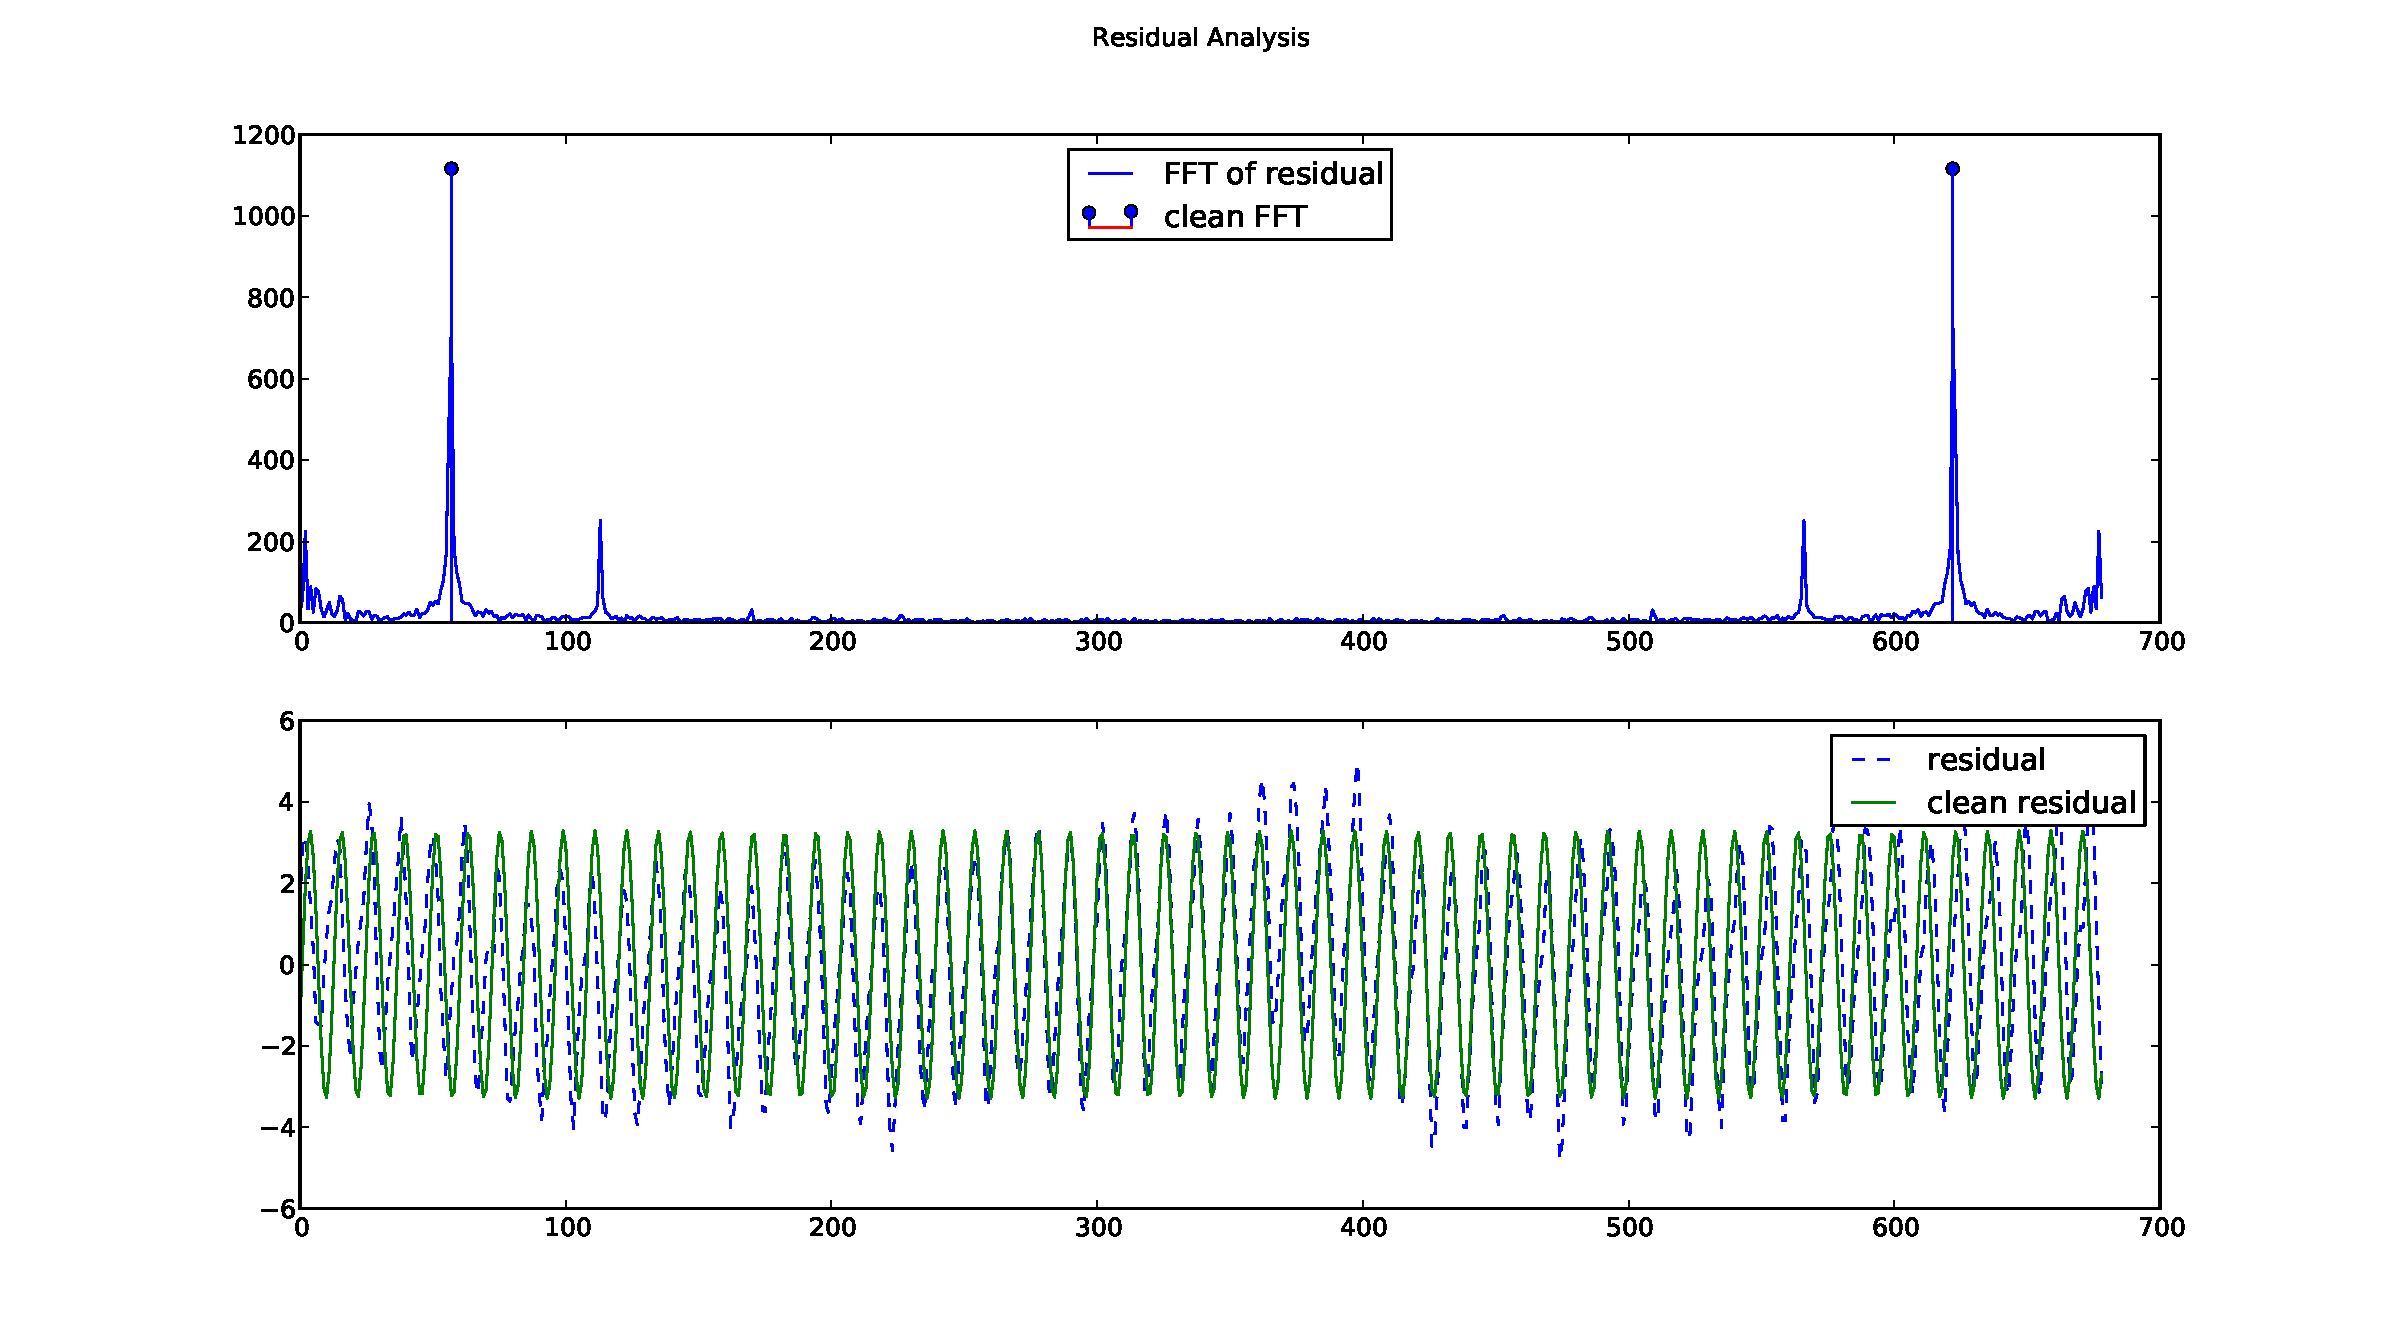
\includegraphics[width=18cm]{figs/co2_spectrum.pdf}
\caption[]{Spectrum of the residual (short-term trend) = $f_{CO_2}(t) - f_L(t)$.}
\label{fig:co2_spectrum}
\end{subfigure}\\
\begin{subfigure}[h]{\linewidth}
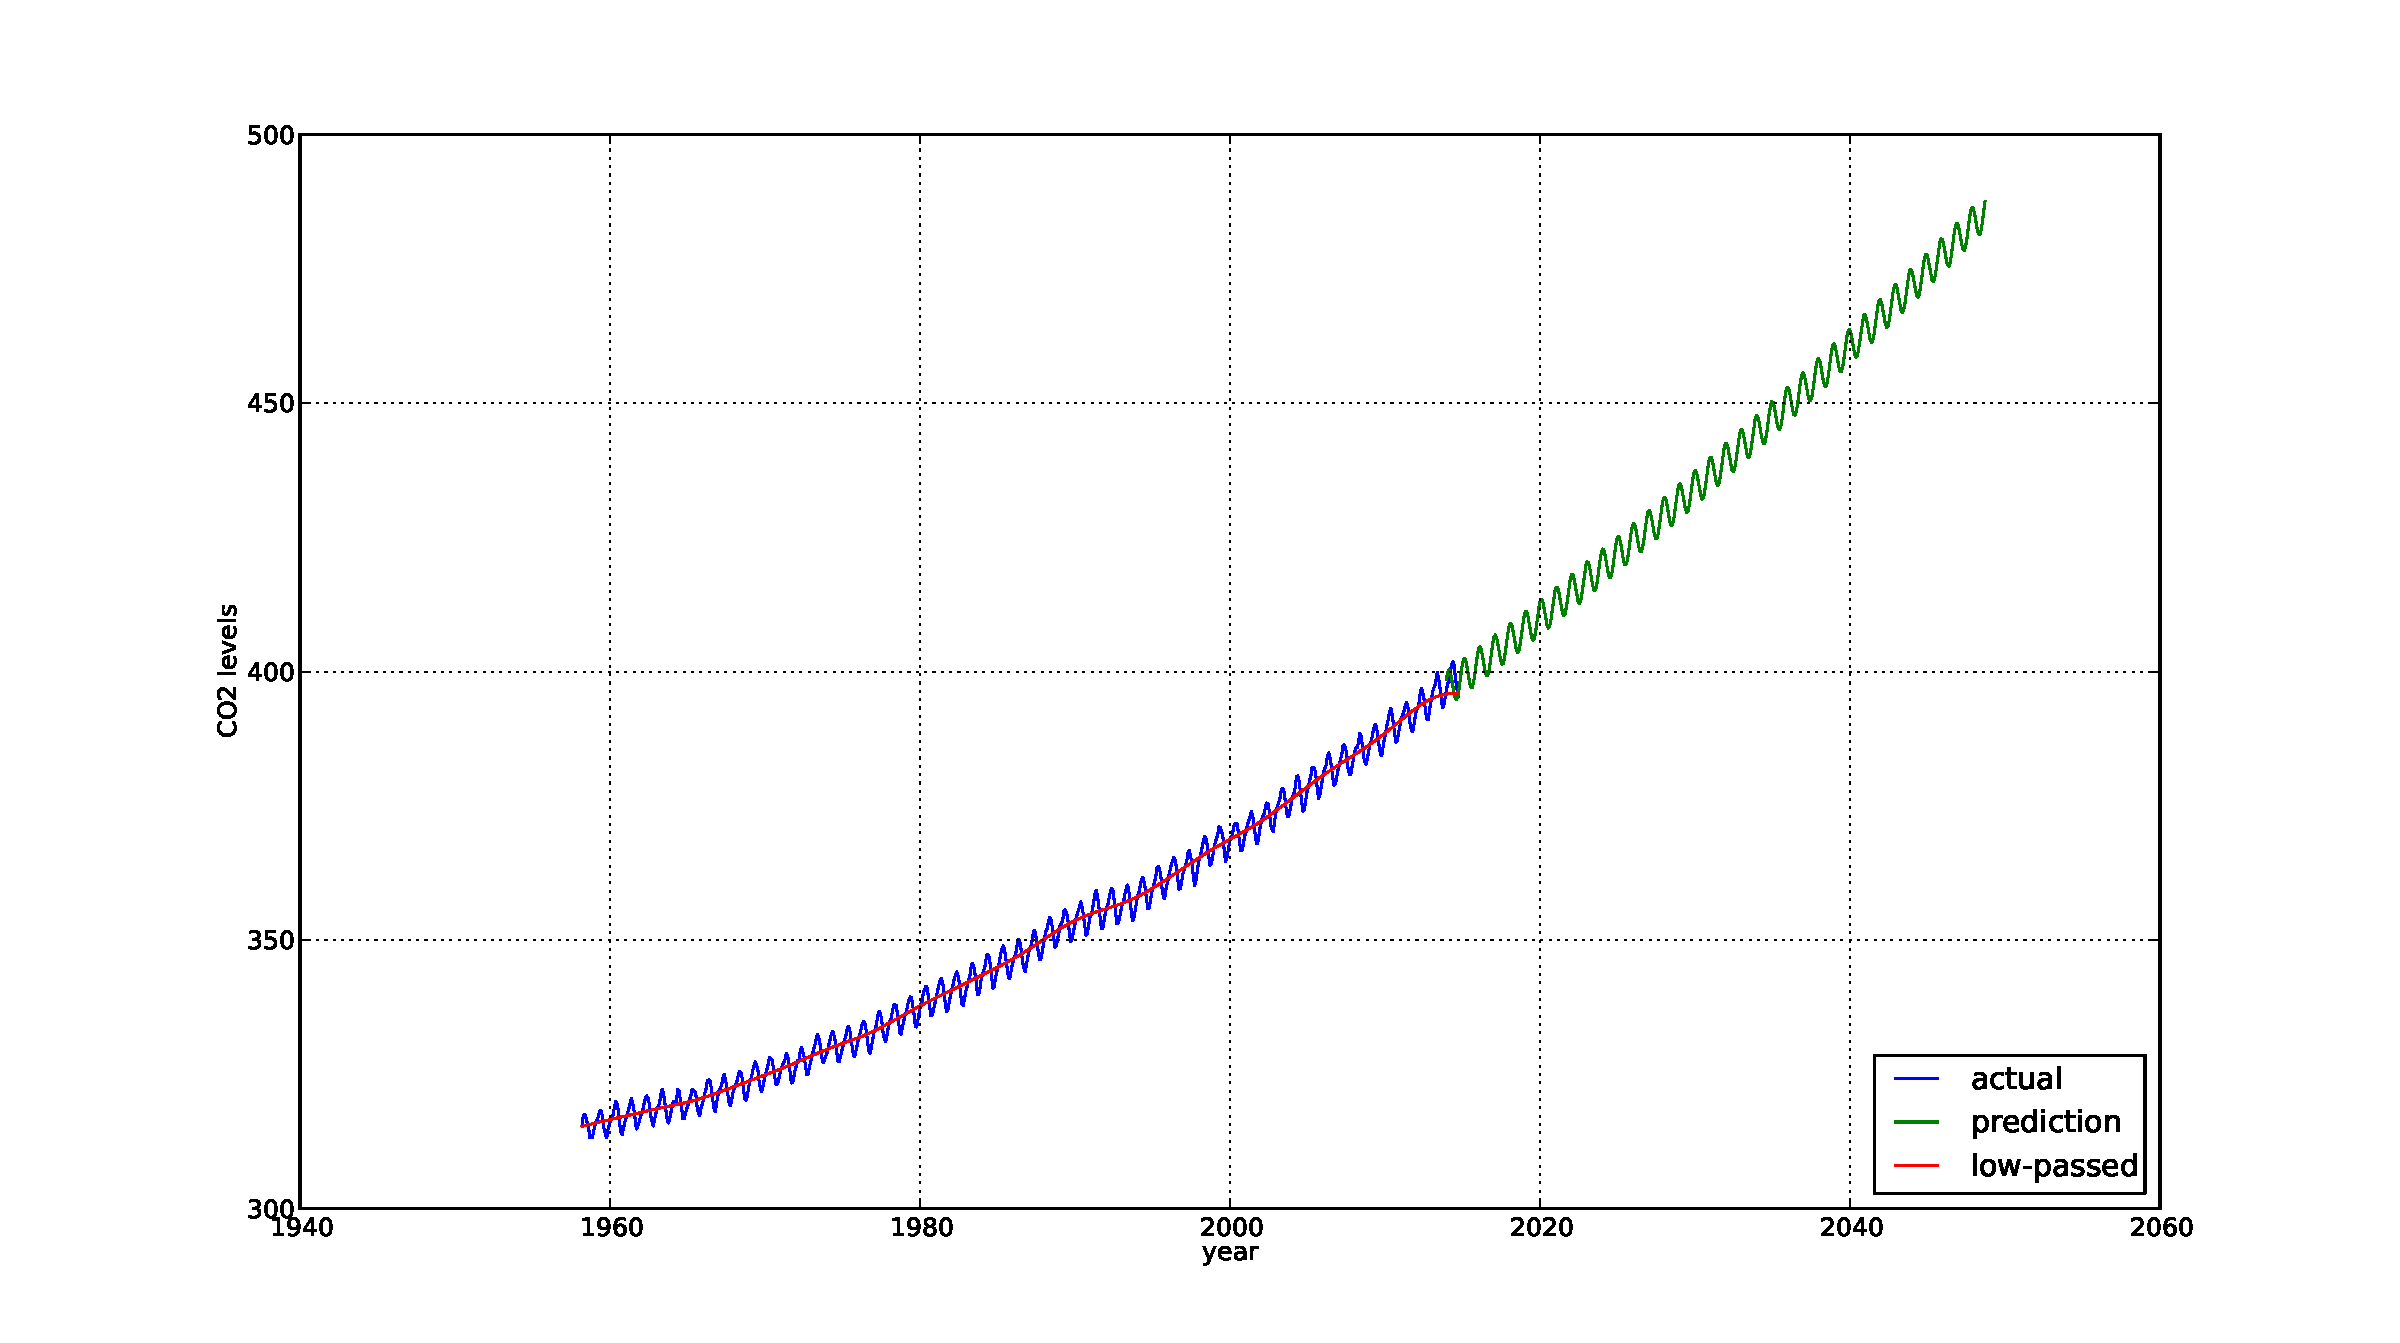
\includegraphics[width=18cm]{figs/co2_predict.pdf}
\caption[]{Prediction of $\text{CO}_2$ time series data.}
\label{fig:co2_decomp}
\end{subfigure}
\end{center}
\end{figure}

Figure~\ref{fig:co2_decomp} shows the final result --- predictions up to the year 2050. Also shown is the low-passed version of the original signal used for fitting the long-term trend.
\clearpage



In this lab we investigate using Gaussian Processes for regression on weather data prediction. Following are the main features of this implementation.
\begin{itemize}
    \item The code was implemented in Python.
    \item Two mean functions were analyzed : (1) constant mean = mean of the data (2) cubic spline fit to the data.\footnote{ Note that these are strictly not bayesian methods as we are using the data itself to specify the prior.}
    \item Two covariance functions were analyzed :
        \begin{enumerate}
        \item Squared-Exponential = $\sigma^2 exp\left(-\dfrac{(x_1-x_2)^TM^{-1}(x_1-x_2}{2}\right) + \sigma_y^2I$
        \item Periodic  = $\sigma^2 exp\left(-l^2\sin^2(2\pi/b|x_1-x_2|)\right)$
        \end{enumerate}
        \item The hyperparameters were tuned by maximizing the marginal likelihood. Analytical gradients were used with the conjugate gradient optimization method.
        \item Sequential predictions were also carried out for Tide Height and Temperature time series.
\end{itemize}
\textbf{Please note all figures indicate intervals of 1 and 2 standard deviations.}
\subsection*{RMS Error with Different Means/ Covariances}
The table below indicates the root-mean-squared error of the \textbf{tide-height} predcitions with respect to the ground-truth data. The covariance hyper-parameters used for these experiments were optimised through marginal likelihood as detailed in the next section.

\begin{table}[h]
\begin{center}
\begin{tabular}{|l||r|r|r|r|r|r|r|r|r|r|r|}
\hline
Mean \textbackslash Covariance & Squared-Exponent & Periodic\\\hline\hline
Mean(data) & \textbf{0.158} &   0.175 \\\hline
Spline     & 0.240 &   0.290 \\\hline
\end{tabular}
\caption{RMS Error for tide-height predictions.}
\label{tab1}
\end{center}
\end{table}

%\begin{figure}[h]
%\begin{subfigure}[h]{\linewidth}
%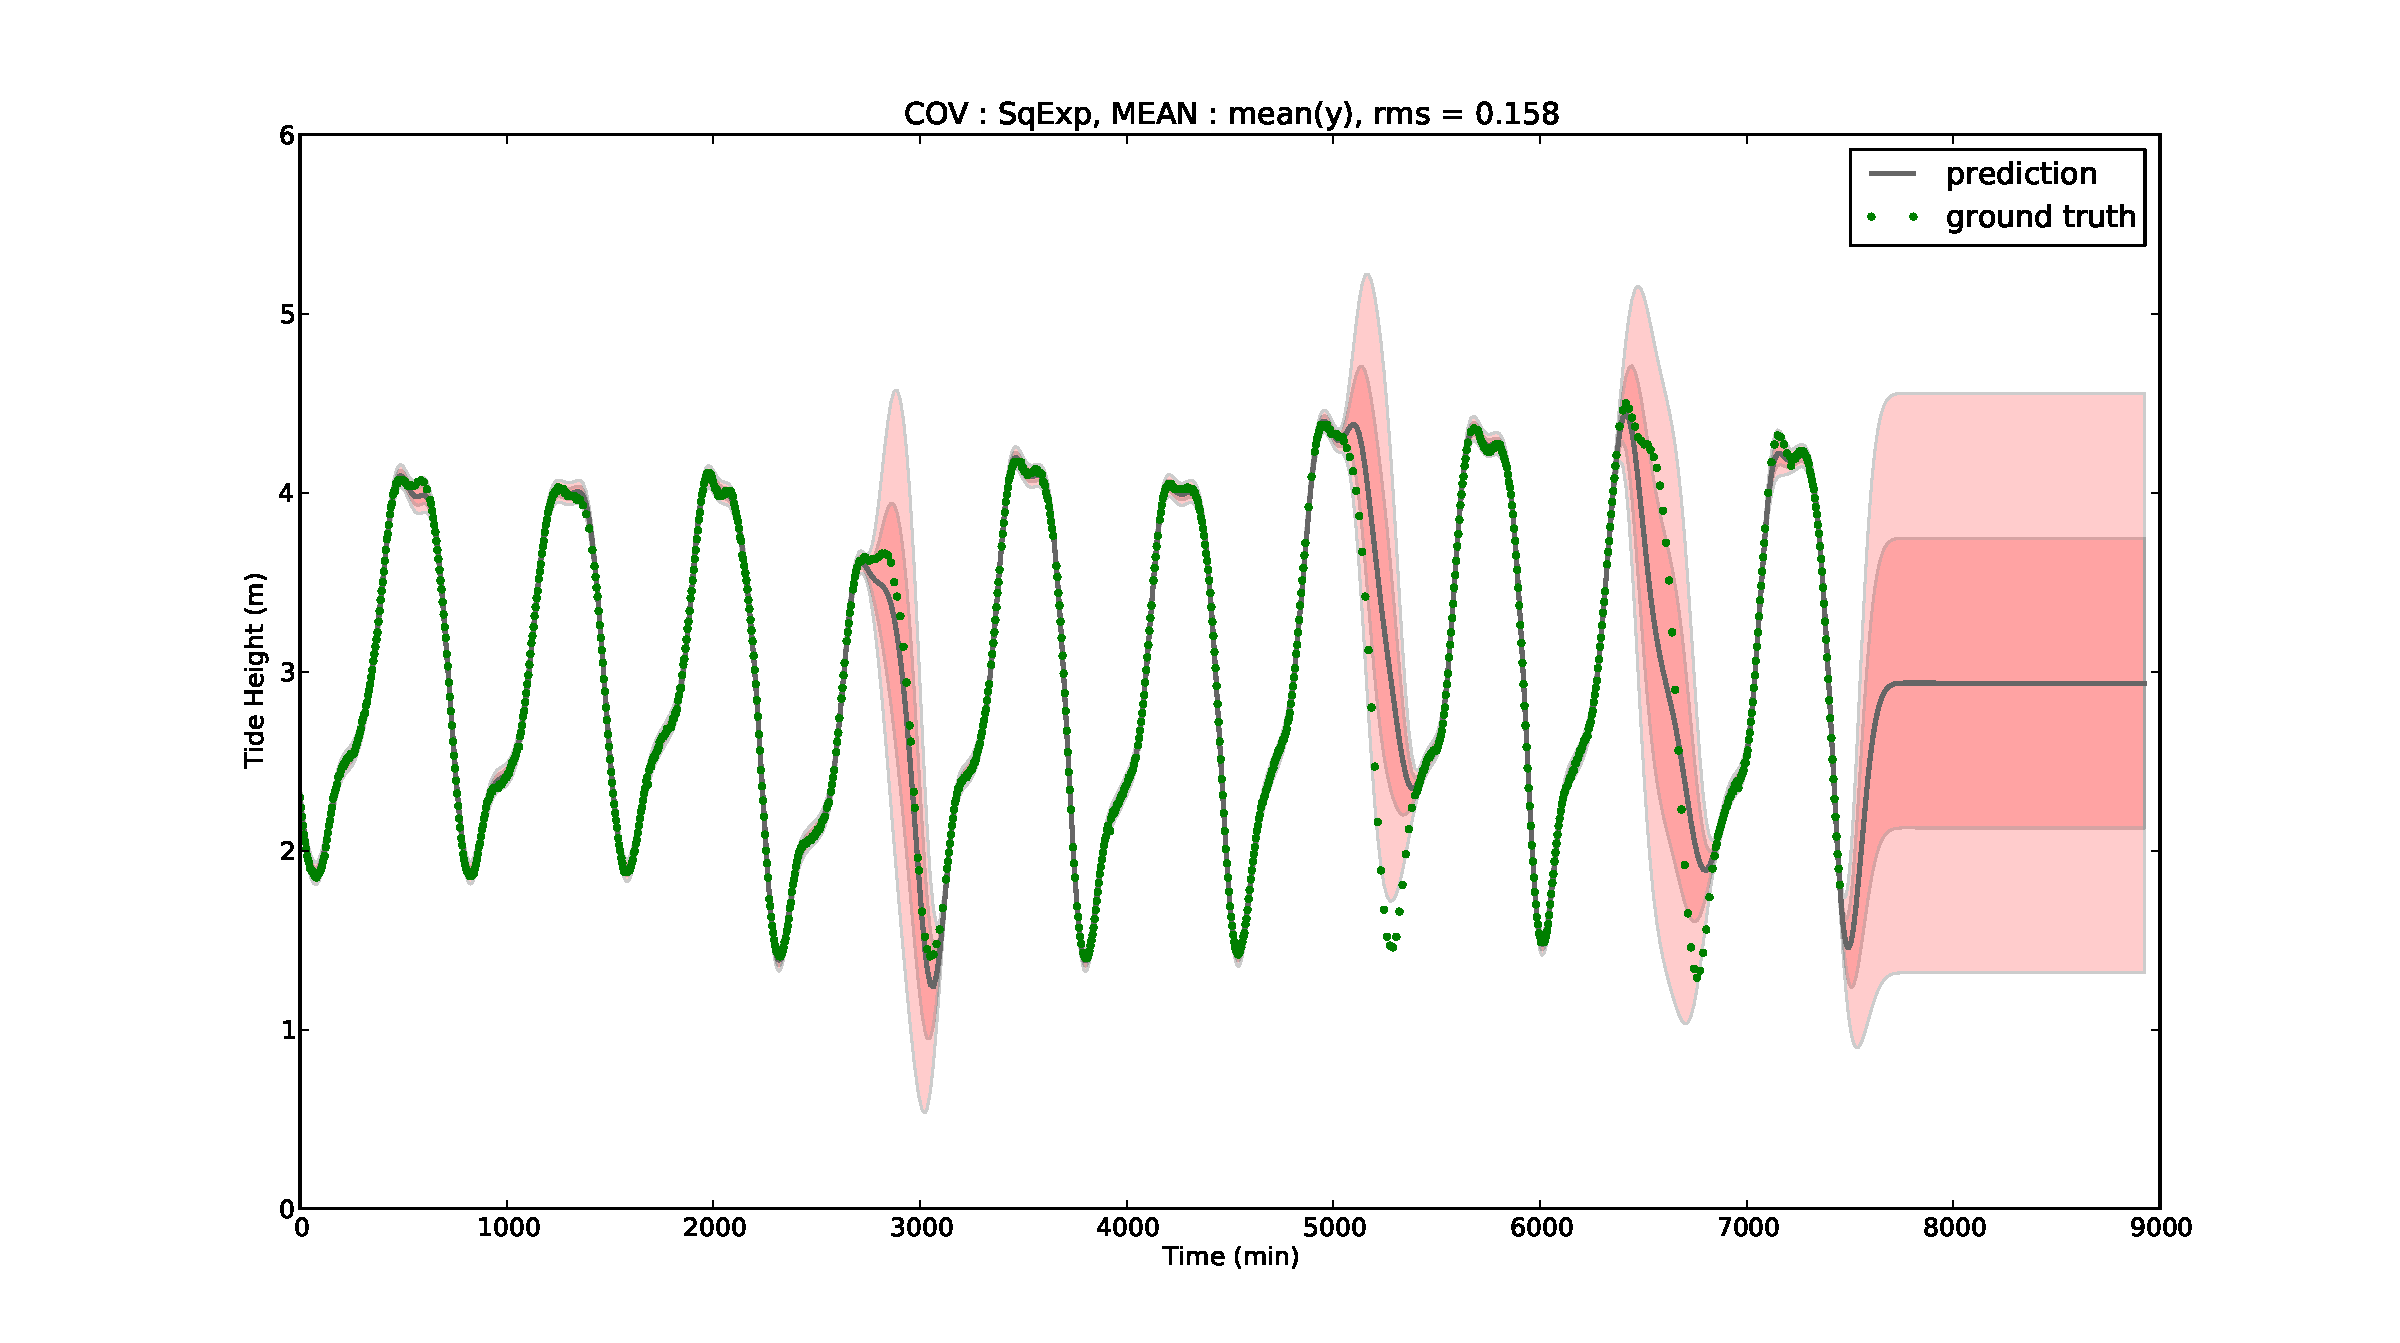
\includegraphics[width=15cm, height=6.5cm]{figs/h_sqexp_const.pdf}
%\caption{}
%\end{subfigure}\\
%\begin{subfigure}[h]{\linewidth}
%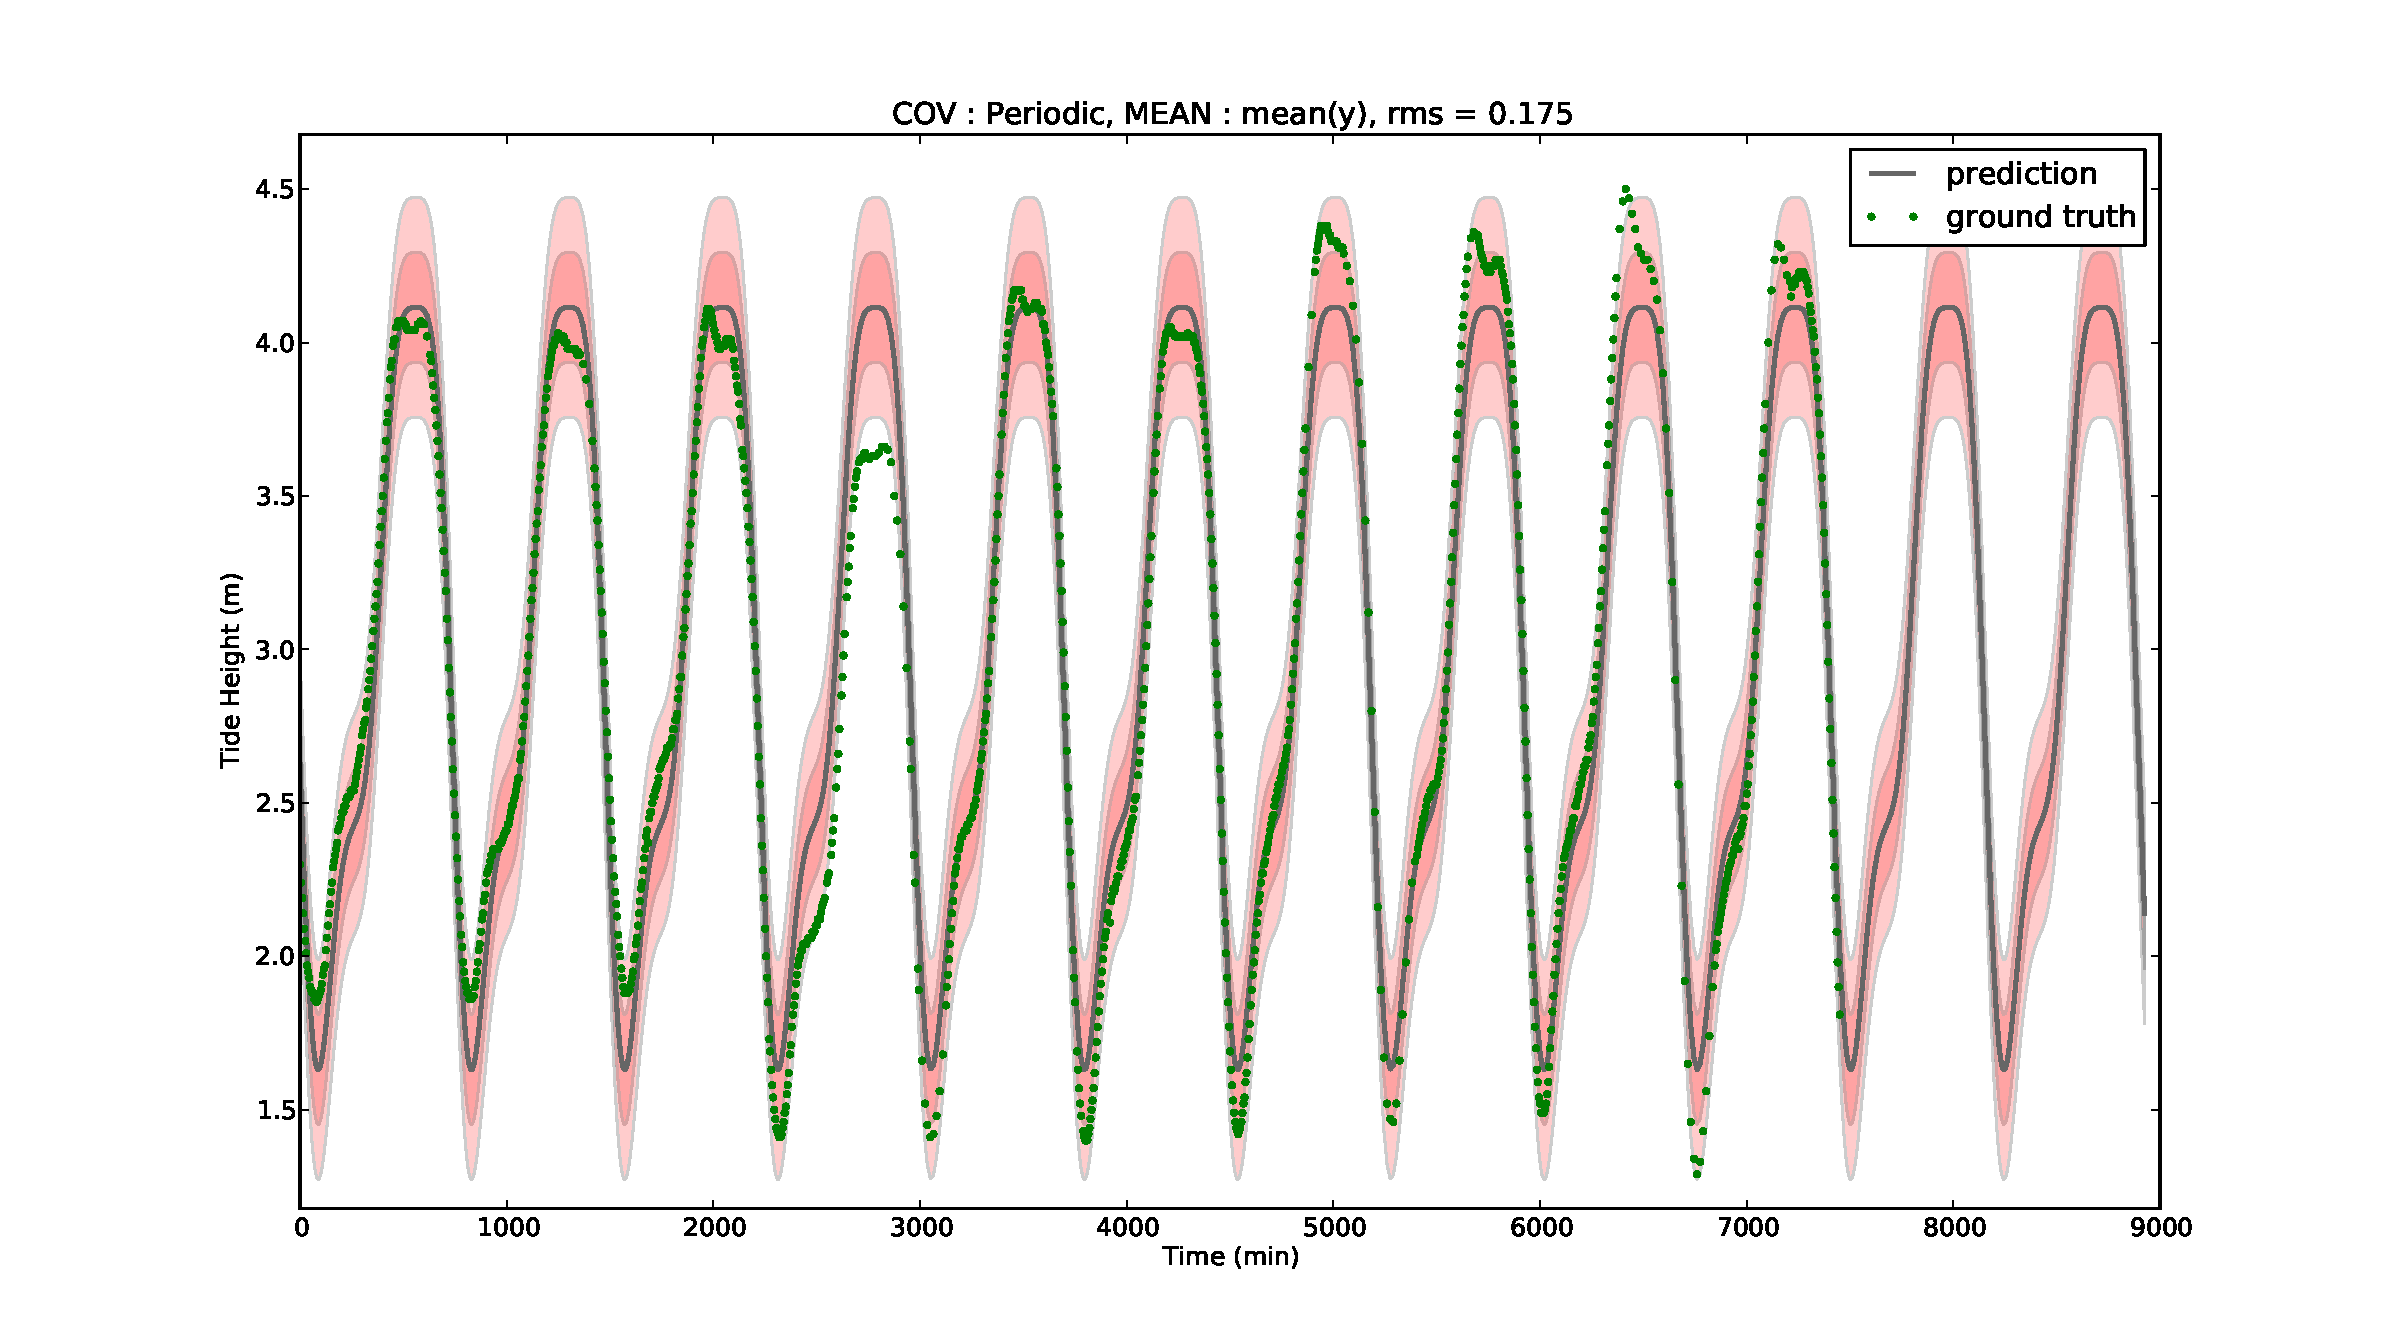
\includegraphics[width=15cm, height=6.5cm]{figs/h_per_const.pdf}
%\caption{}
%\end{subfigure}%
%\caption[]{The figure (a) above uses the square-exponential covariance where as figure (b) uses periodic (sin-squared-exponent). Even though the rms error of (a) is lower than (b) (0.158 < 0.175), notice the variance towards the end (after $t>7000$) --- the variance for the squared-exponent is higher than periodic kernel because it cannot capture the long-term periodic trend in the data.}
%\label{fig:f1}
%\end{figure}
%\clearpage

\end{document}
